
%(BEGIN_QUESTION)
% Copyright 2013, Tony R. Kuphaldt, released under the Creative Commons Attribution License (v 1.0)
% This means you may do almost anything with this work of mine, so long as you give me proper credit

This audio amplifier circuit uses a coupling capacitor ($C_3$) and a transformer ($T_1$) to transfer power to an 8-ohm audio speaker:

$$\includegraphics[width=15.5cm]{i03376x01.eps}$$

Calculate the reactance of $C_3$ at a signal frequency of 5.4 kHz, and also identify the purpose of the transformer in this circuit.

\vskip 20pt

$X_C$ = 

\vskip 20pt

\noindent
The purpose of transformer $T_1$ is to (choose one answer):
\vskip 5pt
\item{} Prevent transistor $Q_1$ from saturating from excess signal levels
\vskip 5pt
\item{} Match the amplifier's output impedance to the speaker's load impedance
\vskip 5pt
\item{} Step up the amplifier's output signal voltage for better audio quality
\vskip 5pt
\item{} Compensate for temperature changes affecting transistor beta ratio
\vskip 5pt
\item{} Step down AC line voltage to a safe level to power the amplifier
\vskip 5pt
\item{} Convert AC into DC so that the amplifier may function on AC power
\end{itemize}


\underbar{file i03376}
%(END_QUESTION)





%(BEGIN_ANSWER)

$X_C$ = 0.8931 $\Omega$

\vskip 10pt

\item{} Match the amplifier's output impedance to the speaker's load impedance

%(END_ANSWER)





%(BEGIN_NOTES)

{\bf This question is intended for exams only and not worksheets!}.

%(END_NOTES)


